\section{Materials and Methods}\label{Materials and Methods}
\begin{figure*}[htbp]
    \centering
    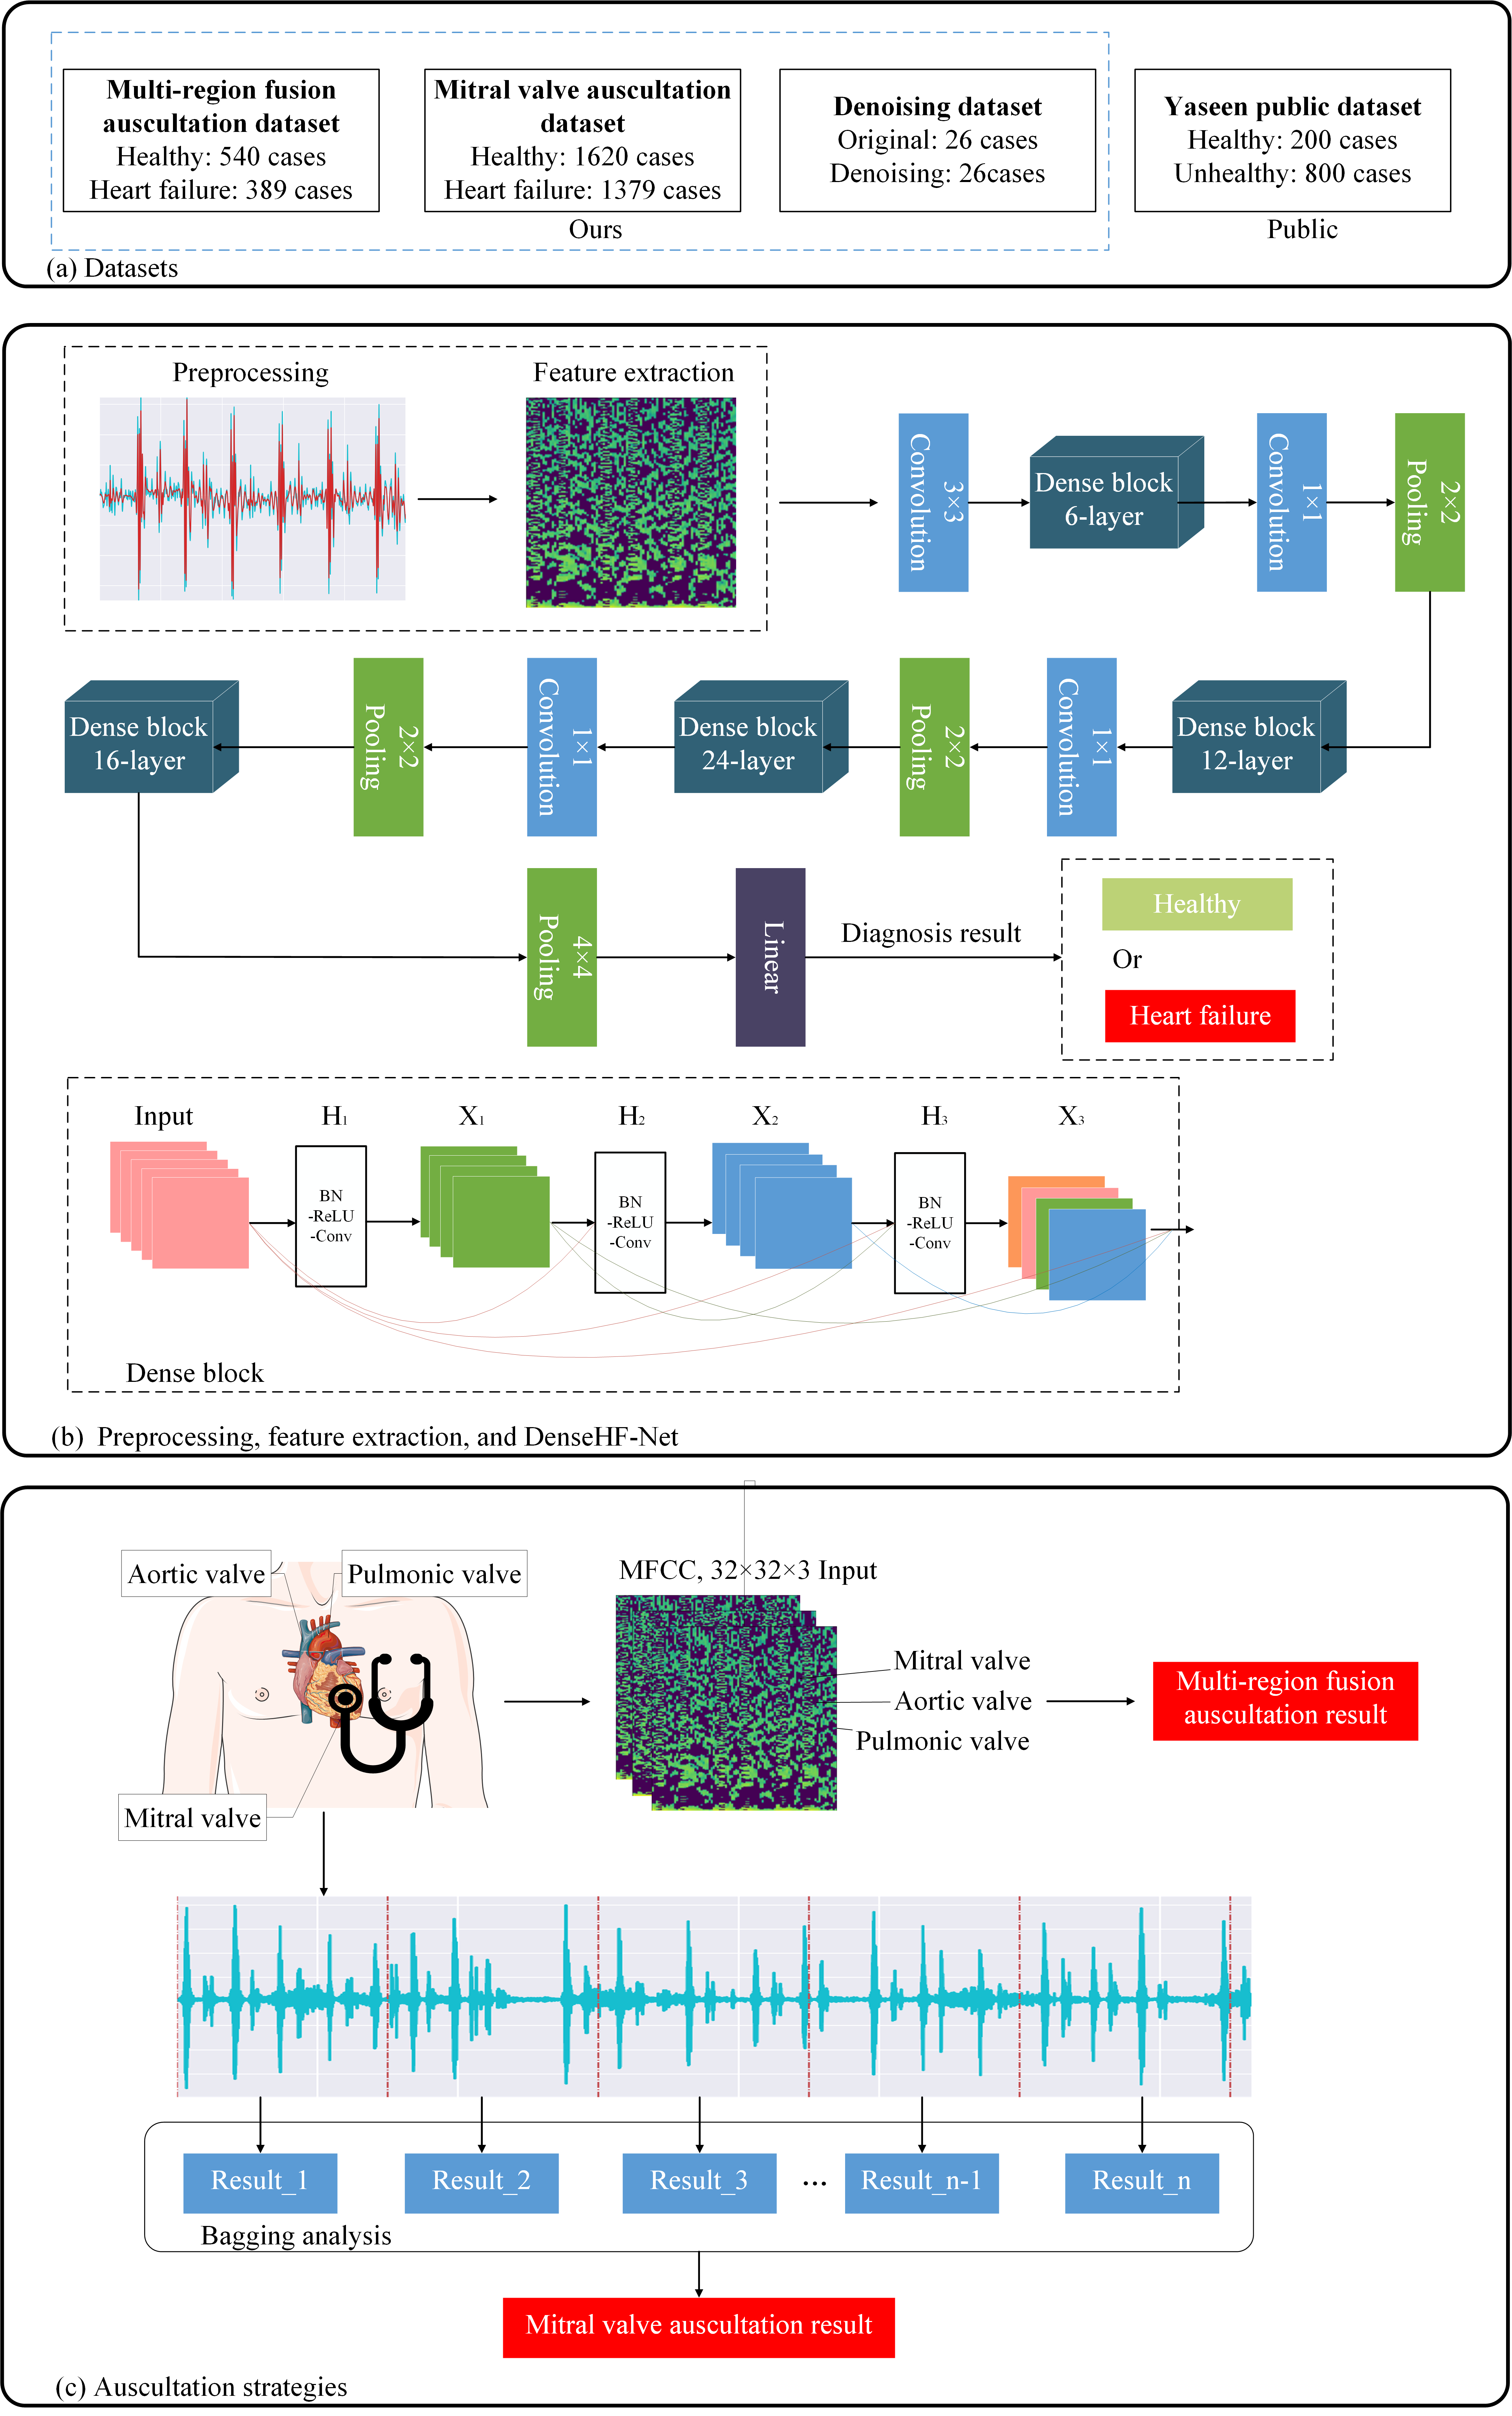
\includegraphics[width=0.8\linewidth]{figs/methods/all.png}
    \caption{\textbf{Methodology of the proposed work.} (\textbf{a}) A dataset was built in this paper, including two HF diagnostic subsets, a denoising subset, and a public subset. (\textbf{b}) The layered architecture of the proposed DenseHF-Net contains four Dense blocks. (\textbf{c}) Multi-region fusion auscultation and mitral valve auscultation.}
	\label{FIG:Methodology}
\end{figure*}
Fig. \ref{FIG:Methodology} illustrates the methodology employed in this paper. Firstly, in order to address the data scarcity issue in the development of AHF diagnostic models, we have created several datasets. We create a multi-region fusion auscultation dataset, containing 540 healthy cases and 389 heart failure cases. Each case includes three audio recordings corresponding to the mitral valve, aortic valve, and pulmonic valve. Additionally, a mitral valve auscultation dataset is established, containing 1620 healthy cases and 1379 heart failure cases, with each recording lasting between three to five seconds.

Next, in response to the signal processing and lightweight requirements for rapid AHF diagnosis, we have developed a wavelet denoising algorithm and a lightweight DenseHF-Net. We explore a wavelet denoising algorithm specifically designed for short-duration heart sound signals to reduce noise effectively. Subsequently, we employ the MFCC algorithm to extract one-dimensional sound signals into two-dimensional image features. Finally, a DenseHF-Net is used to train on the MFCC features.

Two distinct auscultation strategies are introduced in this paper.  1. Multi-region fusion auscultation is designed for
scenarios where long-time auscultation is possible, using the fusion characteristics of the mitral valve, aortic valve, and pulmonic valve as input features. 2. Mitral valve auscultation is specifically
designed for AHF rapid diagnosis in cases of ambulances. In the case of mitral valve auscultation lasting more than 10 seconds, an ensemble method is proposed. 
\subsection{Datasets}
\subsubsection{HF auscultation datasets}
The heart sound databases were acquired at Tianjin 4th Center Hospital of China between 2021 and 2022. The data were recorded using a 3M™ Littmann® electronic stethoscope 3200, with a sampling rate set at 22kHz. This project was approved by the medical ethics committee of Tianjin 4th Center Hospital of China (No. 2022-T050). All volunteers have signed an informed consent. 

Under the guidance of two chief physicians, we collected heart sounds from heart failure patients in various departments to create a pathological dataset. We recruited volunteers among patients diagnosed with heart failure, recorded auscultation at three different regions, and simultaneously documented their gender, age, hospitalization information, medical history, and the latest biochemical markers. Afterward, the chief physicians reviewed the data to exclude samples that had already recovered from heart failure or had unclear signs of heart failure features. Finally, heart sounds from a healthy population were collected in the same manner to serve as a comparison group. As shown in Tab. \ref{tab: Results, Datasets}, the HF auscultation dataset consists of a total of 71.6 minutes of heart failure auscultation and 81 minutes of the comparison group auscultation.

The multi-region fusion auscultation dataset comprises 540 healthy cases and 389 cases of heart failure. Each case includes three audio recordings of the mitral valve, aortic valve, and pulmonic valve. To ensure robustness, we established a 10-fold cross-validation database after shuffling.

The mitral valve auscultation dataset consists of 1620 healthy cases and 1379 cases of heart failure, with each case featuring audio recordings lasting three to five seconds. Similar to the previous dataset, we created a 10-fold cross-validation database after shuffling.
\subsubsection{Denoising dataset}
As shown in Fig. \hyperref[FIG:Methodology]{1a}, we have created a comparative dataset before and after denoising, encompassing 26 different pathological descriptions. The initial 26 recordings are characterized as noisy signals, encompassing various common abnormal heart sounds. In contrast, the remaining 26 control recordings were subsequently reviewed and verified by two medical professionals to eliminate background noise while preserving all relevant pathological information.
\subsubsection{Yaseen public dataset}
As shown in Fig. \hyperref[FIG:Methodology]{1a}, we also use a publicly available Yaseen dataset \cite{son2018classification}. This dataset includes Aortic Stenosis (AS), Mitral Regurgitation (MR), Mitral Stenosis (MS), Mitral Valve Prolapse (MVP), and Normal (N). The main purpose is to evaluate the model's generalization ability in diagnosing normal and abnormal heart sounds. We employ 80\% training data and 20\% testing data. Each case is recorded for a duration of 2 seconds.
\subsection{Preprocessing}
The preprocessing of heart sound signals aims to depress the noisy background in clinical environments. Wavelet transform is used to decrease the noise of heart sounds based on mother wavelets, such as Haar, db, Coif, Sym, and Biorthogonal (bior). Chen et al. \cite{2006Research} achieved optimal denoising results using the db6 wavelet basis. Zhao et al. \cite{2010Research} reported the best outcomes with the bior5.5 basis. Cheng et al. \cite{cheng2014denoising} utilized wavelet-based adaptive algorithms to enhance the denoising of heart signals, resulting in a signal improvement of 12.4 dB compared to the pre-denoising state.
% The assessment of denoising effectiveness is often based on evaluation indices like the signal-to-noise ratio (SNR), calculated using the formula Eq.(\ref{eq:SNR}).
% \begin{equation}
% 	\begin{aligned}
% SNR_{db} = 10 \log_{10} \frac{P_{signal}}{P_{noise}}
% \label{eq:SNR}
% 	\end{aligned}
% \end{equation}

In this paper, we consider three wavelet functions: db6, sym8, and coif5. These wavelet bases are used for the discrete wavelet decomposition of heart sound recordings. Following the decomposition, discrete wavelet reconstruction is performed, with a coefficient shrinkage function applied at a threshold of 20\% modulo the maximum hard threshold.

Secondly, in order to determine the coefficient contraction strategy, various coefficient contraction functions are applied during both the discrete wavelet decomposition and reconstruction processes. 

We introduce a novel self-adaptive threshold function, as depicted in Eq.(\ref{eq:self}).
\begin{equation}
f_{self}(x,T)=
	\begin{cases}
	e^{\frac{x+T}{2}}-e^{\frac{-x-T}{2}}&x \leq -T\\ 
	0& -T \leq x \leq T\\
	e^{\frac{x-T}{2}}-e^{\frac{-x+T}{2}}&x \geq T
	\end{cases}
	\label{eq:self}
\end{equation}

$f_{self}$ has the following three advantages:
\begin{itemize}
\item $f_{self}$ satisfies: $$\lim_{x \to -T^-}f_{self}(x)=\lim_{x \to -T^+}f_{self}(x)=0$$ $$\lim_{x \to T^-}f_{self}(x)=\lim_{x \to T^+}f_{self}(x)=0$$ 

$f_{self}$ is differentiable at $x=\pm T$
\item $f_{self}$ is odd, with smooth and monotonically increasing curves.
\item $f_{self}$ can overcome the problem of discontinuities in the hard threshold function so that the reconstructed signal retains more detailed information after the reconstruction.
\end{itemize}

We collect statistical data on the average signal-to-noise ratio (SNR) under different coefficient contraction functions and thresholds.
\subsection{Feature extraction}
Feature extraction for heart sound signals aims to reduce the dimensionality of the data, highlight key information, and thereby improve the subsequent data processing and analysis. Mel Spectrum and MFCC have widely employed feature extraction methods in speech recognition. Human perception of frequency is non-linear, with greater sensitivity to low-frequency signals compared to high-frequency ones. Consequently, frequency conversion is performed according to the equation Eq.(\ref{eq:melscale}).
\begin{equation}
	\begin{aligned}
Mel(f)=2595\ln \left(1+\frac{f}{700} \right)
\label{eq:melscale}
	\end{aligned}
\end{equation}

To reproduce the Meier scale in the processing of discrete digital signals, the power spectral estimates of the resulting periodic plot are filtered using a Mehr filter bank (usually 26 V-Band Pass filter banks), as shown in Eq.(\ref{eq:melbank}).
\begin{equation}
H_m(k)=
	\begin{cases}
	\frac{k-f(m-1)}{f(m)-f(m-1)} & f(m-1)\leq k \leq f(m)\\
	\frac{f(m+1)-k}{f(m+1)-f(m)} & f(m)\leq k \leq f(m+1)\\
	{0} & others
	\end{cases}
	\label{eq:melbank}
\end{equation}

Multiply with FFT to get the Mel spectrum:Eq. (\ref{eq:melspec}).
\begin{equation}
MelSpec(m)=\sum\limits_{k=f(m-1)}\limits^{f(m+1)}H_m(k)*\left|X(k)\right|^2
	\label{eq:melspec}
\end{equation}

Calculate the logarithmic energy output of the V-Band Pass filter bank: Eq.(\ref{eq:eninge}). Discrete cosine transform (DCT): Eq. (\ref{eq:DCT}) to obtain the MFCC coefficient.
\begin{equation}
S(m)=\ln \left( {\sum\limits_{k=0}\limits^{N-1})\left|X_a(k)\right|^2H_m(k)}\right),
0 \leq m \leq M
	\label{eq:eninge}
\end{equation}

\begin{equation}
C(n)=\sum\limits_{m=0}\limits^{N-1}S(m) \cos \left( {\frac{\pi n(m-0.5)}{M}}\right)
,n=1,2,...,L
	\label{eq:DCT}
\end{equation}
The L order refers to the order of the MFCC coefficient, usually 12-16. M is the number of triangular filters.

The MFCC feature design in this paper is defined as Wu et al. \cite{wu2010hidden} and has achieved the same time-frequency extraction effect as Vepa \cite{vepa2009classification}, as shown in Fig. \hyperref[FIG:Methodology]{1a}.
\subsection{DenseHF-Net}
\begin{table*}[width=2\linewidth]
\caption{Models parameter setting}
\label{tab:Modesl Parameters Setting}
\begin{tabular*}{\tblwidth}{CCC|CCC|CCC}
\toprule
\multicolumn{3}{c}{\textbf{DenseHF-Net (ours)}}&\multicolumn{3}{c}{\textbf{ResNet-18} \cite{he2016deep}}&\multicolumn{3}{c}{\textbf{MobileNetV1-28} \cite{howard2017mobilenets}}\\
\multicolumn{3}{c}{\textbf{Number of parameters: }0.33M}&
\multicolumn{3}{c}{\textbf{Number of parameters: }42.61M}&
\multicolumn{3}{c}{\textbf{Number of parameters: }12.24M}\\
\multicolumn{3}{c}{\textbf{Memory access cost: }30.64M}&
\multicolumn{3}{c}{\textbf{Memory access cost: }556.97M}&
\multicolumn{3}{c}{\textbf{Memory access cost: }46.28M}\\
\multicolumn{3}{c}{\textbf{Forward/backward pass size: }20.18M}&
\multicolumn{3}{c}{\textbf{Forward/backward pass size: }13.63M}&
\multicolumn{3}{c}{\textbf{Forward/backward pass size: }10.31M}\\
% \cmidrule{1-3}\cmidrule{4-6}\cmidrule{7-9}
Layer&Filters&Output&Layer&Filters&Output&Layer&Filters&Output\\ 
\hline
Feature Map&$\begin{bmatrix}3\times3,24\end{bmatrix}\times1$&$32\times32$&
Feature Map&$\begin{bmatrix}3\times3,64\end{bmatrix}\times1$&$32\times32$&
Feature Map&$\begin{bmatrix}3\times3,32\end{bmatrix}\times1$&$30\times30$\\ 
% \cmidrule{1-3}\cmidrule{4-6}\cmidrule{7-9}
Dense Block& $\begin{bmatrix}1\times1,48\\3\times3,12\end{bmatrix}\times4$ &$32\times32$&
Conv2\_x& $\begin{bmatrix}3\times3,64\\3\times3,64\end{bmatrix}\times2$& $32\times32$&
Conv\_dw,pw&$\begin{bmatrix}3\times3,32\\1\times1,64\end{bmatrix}\times1$ & $30\times30$\\ 
% \cmidrule{1-3}\cmidrule{4-6}\cmidrule{7-9}
Transition& $\begin{bmatrix}1\times1,conv\\2\times2,pool\end{bmatrix}$&$16\times16$&
Conv3\_x& $\begin{bmatrix}3\times3,128\\3\times3,128\end{bmatrix}\times2$& $16\times16$&
Conv\_dw,pw&$\begin{bmatrix}3\times3,64\\1\times1,128\end{bmatrix}\times1$ & $15\times15$\\ 
% \cmidrule{1-3}\cmidrule{4-6}\cmidrule{7-9}
Dense Block& $\begin{bmatrix}1\times1,48\\3\times3,12\end{bmatrix}\times8$ &$16\times16$&
Conv4\_x& $\begin{bmatrix}3\times3,256\\3\times3,256\end{bmatrix}\times2$& $8\times8$&
Conv\_dw,pw&$\begin{bmatrix}3\times3,128\\1\times1,128\end{bmatrix}\times1$ & $15\times15$\\
% \cmidrule{1-3}\cmidrule{4-6}\cmidrule{7-9}
Transition& $\begin{bmatrix}1\times1,conv\\2\times2,pool\end{bmatrix}$&$8\times8$&
Conv5\_x& $\begin{bmatrix}3\times3,512\\3\times3,512\end{bmatrix}\times2$& $4\times4$&
Conv\_dw,pw&$\begin{bmatrix}3\times3,128\\1\times1,256\end{bmatrix}\times1$ & $8\times8$ \\ 
% \cmidrule{1-3}\cmidrule{4-6}\cmidrule{7-9}
Dense Block& $\begin{bmatrix}1\times1,48\\3\times3,12\end{bmatrix}\times16$ &$8\times8$&
Pooling& $4\times4$& $1\times1\times512$&
Conv\_dw,pw&$\begin{bmatrix}3\times3,256\\1\times1,256\end{bmatrix}\times1$ & $8\times8$\\
% \cmidrule{1-3}\cmidrule{4-6}\cmidrule{7-9}
Transition& $\begin{bmatrix}1\times1,conv\\2\times2,pool\end{bmatrix}$&$4\times4$&
Linear& & $1\times2$&
Conv\_dw,pw&$\begin{bmatrix}3\times3,256\\1\times1,512\end{bmatrix}\times1$ & $4\times4$\\ 
% \cmidrule{1-3}\cmidrule{4-6}\cmidrule{7-9}
Dense Block& $\begin{bmatrix}1\times1,48\\3\times3,12\end{bmatrix}\times8$ &$4\times4$&
&&&
Conv\_dw,pw&$\begin{bmatrix}3\times3,512\\1\times1,512\end{bmatrix}\times5$ & $4\times4$\\
% \cmidrule{1-3}\cmidrule{7-9}
Pooling& $4\times4$& $1\times1\times384$&
&&&
Conv\_dw,pw&$\begin{bmatrix}3\times3,512\\1\times1,1024\end{bmatrix}\times1$ & $2\times2$\\
% \cmidrule{1-3}\cmidrule{7-9}
Linear& & $1\times2$&
  & & &
Conv\_dw,pw&$\begin{bmatrix}3\times3,1024\\1\times1,1024\end{bmatrix}\times1$ & $2\times2$\\
% \cmidrule{1-3}\cmidrule{7-9}
&&&
  & & &
Pooling& $2\times2$& $1\times1\times1024$\\
% \cmidrule{7-9}
&&&
  & & &
Linear& & $1\times2$\\
\bottomrule
\end{tabular*}
\end{table*}
The common deep learning model architecture for heart sound diagnosis includes Convolutional Neural Networks (CNN), Recurrent Neural Networks (RNN), Long Short-Term Memory networks (LSTM), and Convolutional Neural Network-Long Short-Term Memory network hybrids (CNN-LSTM) \cite{rubin2016classifying,arora2021transfer,li2021lightweight,shuvo2021cardioxnet}. This paper focuses on model design specifically tailored for AHF rapid diagnosis, aiming to develop a model that balances lightweight characteristics with accuracy.

We introduce DenseHF-Net, which is based on the CVPR 2017 Best Paper, Dense-Net \cite{huang2017densely}. 
To achieve model lightweight, DenseHF-Net employs only four Dense Blocks: DenseBlock-1, DenseBlock-2, DenseBlock-3, and DenseBlock-4. This choice reduces the model's parameter count and computational load while still maintaining a certain level of depth and feature extraction capability. Three transition layers with small compression rates are employed simultaneously to reduce the output channel numbers of the 1x1 convolutional layers, thereby reducing the size of feature maps. Ultimately, the diagnostic results are obtained after passing through a linear layer. The parameter settings for the three models are detailed in Tab. \ref{tab:Modesl Parameters Setting}.

The classic ResNet \cite{he2016deep} and MobileNet \cite{howard2017mobilenets} models are also trained for comparison with DenseHF-Net. All input features are resized to $32\times32$ to make it more convenient for mobile terminals. The parameter numbers of the three models are 3.82M, 42.61M, and 12.24M. The Memory Access Cost (MAC) of the three models are 130.89M, 556.97M, and 46.28M.

% Experimental environment:
% \begin{itemize}
%   \item System: Ubuntu 18.04
%   \item CPU: Intel(R) Core(TM) i7-9700K CPU @ 3.60GHz
%   \item GPU: NVIDIA GeForce RTX 3090 with 24GB VRAM
%   \item CUDA Version: 11.4
%   \item PyTorch Version: 1.10
% \end{itemize}
Experimental environment system: Ubuntu 18.04; CPU: Intel(R) Core(TM) i7-9700K CPU @ 3.60GHz; GPU: NVIDIA GeForce RTX 3090 with 24G VRAM; CUDA Version: 11.4; Pytorch Version:1.10.
\subsection{Auscultation strategies}
The multi-region fusion auscultation strategy is designed for AHF diagnosis in hospitals, with the aim of reducing the door-to-balloon time. Then to reduce the mortality rate and rehospitalization rate of HF patients \cite{fan2021effects}. Heart sound signals are synchronously collected from three regions, including the mitral valve region, aortic valve region, and pulmonic valve region.

The processing pipeline includes three main steps:

1. Applying wavelet transform to the three channels of heart sound to reduce noise.
2. Feature extraction using the MFCC.
3. Fusion of the three MFCC feature sets to produce input of the same dimension as that of the mitral valve auscultation.

The mitral valve auscultation strategy is designed for emergency medical services (EMS) or general screening scenarios, with a stronger emphasis on convenience, aiming to complete the diagnosis within 15 seconds.

As shown in Fig. \hyperref[FIG:Methodology]{1c}, for mitral valve auscultation durations exceeding 10 seconds, there arises the need to address the challenge of reducing false positive diagnoses. To tackle this issue, this research paper introduces an ensemble learning method as a strategic approach.
\begin{equation}
\begin{split}
Result\_i&= \max \limits_{\alpha_{i}}Softmax(\alpha_{i}) \\
&= \max \limits_{\alpha_{i}}\frac{\exp(\alpha_{i})}{\sum_{i=1}^{2} \exp(\alpha_{i})}
	\label{eq:Resulti}
\end{split}
\end{equation} 

Eq.\ref{eq:Resulti} is used to calculate the diagnostic results for a single fragment. $\alpha_{i}$ represents the model output. $Result_{i}$ is 0 for healthy and 1 for heart failure.
\begin{equation}
Output = Result\_1 \lor Result\_2 \lor \cdots \lor Result\_n
\label{eq:Output}
\end{equation} 

Eq.\ref{eq:Output} represents the result of a one-to-one OR operation applied to auscultation segments, designed to minimize the occurrence of false positives. Here, 'n' denotes the number of fragments, typically set to 3.